\documentclass[trans]{beamer}
\usepackage{etex}
\usepackage{amsthm}
\usepackage{xcolor}
\usepackage{wrapfig}
\usepackage{soul}
\usepackage{lipsum}
\usepackage{booktabs}
\usepackage{graphicx}
\usepackage{algorithm}
\usepackage{algorithmic}
\usepackage{answers}
\usepackage[absolute,overlay]{textpos}
\usepackage{verbatim}
\usepackage{fancyvrb}
\usepackage{xspace}
%\usepackage[labelsep=none]{caption}
\usepackage{tikz}
\usepackage{units}
\usepackage{makeidx}
\usepackage{tabularx}
\usepackage{colortbl}
\usepackage{multirow}
\usepackage{calc}
%\usepackage{graphicx}
%\usepackage{array}
%\usepackage[all]{xy}
%%\usepackage{theapa}
%\usepackage{tikz}
%\usetikzlibrary{shapes.geometric} 
%\usetikzlibrary{shadows} 
%\usetikzlibrary{positioning}
%\usepackage{algorithm}
%%\usepackage{algorithmic}
%\usepackage{algorithmic}
%%\usepackage{algpseudocode}
%\usepackage{natbib}
%\usepackage{apalike}
\usepackage{../book/haldefs}

\mode<presentation>
{
%  \usetheme{AnnArbor}
%  \usetheme{Antibes}
%  \usetheme{Bergen}
%  \usetheme{Berkeley}
%  \usetheme{Berlin}
%  \usetheme{Boadilla}
%  \usetheme{boxes}
%  \usetheme{CambridgeUS}
%  \usetheme{Copenhagen}
%  \usetheme{Darmstadt}
%  \usetheme{default}
%  \usetheme{Dresden}
%  \usetheme{Frankfurt}
%  \usetheme{Goettingen}
%  \usetheme{Hannover}
%  \usetheme{Ilmenau}
%  \usetheme{JuanLesPins}
%  \usetheme{Luebeck}
%  \usetheme{Madrid}
%  \usetheme{Malmoe}
%  \usetheme{Marburg}
%  \usetheme{Montpellier}
%  \usetheme{PaloAlto}
%  \usetheme{Pittsburgh}
%  \usetheme{Rochester}
%  \usetheme{Singapore}
%  \usetheme{Szeged}
%  \usetheme{Warsaw}
  \usetheme{Unife}

%\usecolortheme{lily}% 
  % or ...

  \setbeamercovered{transparent}
  % or whatever (possibly just delete it)
}


\usepackage[english]{babel}
% or whatever

%\usepackage[latin1]{inputenc}
% or whatever
\usetikzlibrary{shapes,snakes}
%%% Local Variables: 
%%% mode: latex
%%% TeX-master: "courseml"
%%% End: 

%%%%%%%%%%% COLORS

\definecolor{darkgrey}{rgb}{0.2,0.2,0.2}
\definecolor{grey}{rgb}{0.9,0.9,0.9}
\definecolor{darkblue}{rgb}{0.0,0.0,0.5}
\definecolor{darkpurple}{rgb}{0.4,0.0,0.4}
\definecolor{darkred}{rgb}{0.5,0.0,0.0}
\definecolor{darkorange}{rgb}{0.5,0.45,0.4}
\definecolor{darkgreen}{rgb}{0.0,0.5,0.0}
\definecolor{darkergreen}{rgb}{0.0,0.4,0.0}
\definecolor{lightblue}{rgb}{0.8,0.8,1.0}
\definecolor{lightgreen}{rgb}{0.8,1.0,0.8}
\definecolor{lightred}{rgb}{1.0,0.8,0.8}
\definecolor{lightyellow}{rgb}{1.0,1.0,0.8}
\definecolor{lightorange}{rgb}{1.0,0.9,0.8}
\definecolor{lightgrey}{rgb}{0.96,0.97,0.98}
\definecolor{Sepia}{HTML}{671800}

%%%%%%%%%%%%% FORMATTING
%
%\newcommand*\chapterlabel{}
%\makeatletter
%\titleformat{\chapter}%
%  [block]                                % shape
%  {\gdef\chapterlabel{}
%   \normalfont\sffamily\Huge\bfseries\scshape}            % format applied to label+text
%  {\gdef\chapterlabel{\thechapter~|~}}    % 
%  {0pt}                                  % horizontal separation between label and title body
%  {\begin{tikzpicture}[remember picture,overlay]
%    \node[yshift=-3cm] at (current page.north west)
%      {\begin{tikzpicture}[remember picture, overlay]
%        \draw[fill=lightgreen] (0,0) rectangle
%          (\paperwidth,3cm);
%        \node[anchor=east,xshift=.9\paperwidth,rectangle,
%              rounded corners=20pt,inner sep=11pt,
%              fill=darkergreen]
%              {\color{white}\chapterlabel#1};
%       \end{tikzpicture}
%      };
%   \end{tikzpicture}
%  }% before the title body
%  []%after the title body
%\makeatother 
%%\titlespacing*{\chapter}{0pt}{50pt}{-10pt}
%
%\newcommand{\sectionsize}{}
%\titleformat{\section}%
%  [hang]% shape
%  {\normalfont\Large\itshape}% format applied to label+text
%  {\textcolor{darkergreen}{\makebox[0pt][r]{\thesection\quad }#1}}% label
%  {1em}% horizontal separation between label and title body
%  {}% before the title body
%  []% after the title body
%
%\titleformat{\subsection}%
%  [hang]% shape
%  {\normalfont\large\itshape}% format applied to label+text
%  {\textcolor{darkergreen}{\makebox[0pt][r]{\thesubsection\quad }#1}}% label
%  {1em}% horizontal separation between label and title body
%  {}% before the title body
%  []% after the title body



%%%%%%%%%%% EXERCISE STUFF

\newtheorem{Ex}{Exercise}
\newenvironment{exercises}{\section{Exercises}}{}
% \center\begin{tabular}{c}\hline{\bf\Large Exercises}\\\hline\end{tabular}}{}

%\Newassociation{solution}{Soln}{solutions}
%\Newassociation{hint}{Hint}{solutions}
\newcommand{\prehint}{~[Hint]}
\newcommand{\presolution}{}
\newcommand{\Opensolutionshook}[2]%
  {\Writetofile{#1}{}}
%\renewcommand{\Solnlabel}[1]{%
%  {\Large\linespread{1}%
%  \begin{tabular}{|p{\textwidth}@{}|}%
%    \hline%
%    \emph{Solution #1}\\%
%    \hline%
%  \end{tabular}\newline}}
%\renewcommand{\Hintlabel}[1]{\emph{Hint #1}}


\newcommand{\emptylist}{[ ]}
\newcommand{\pushlist}[1]{{\ensuremath \oplus} #1}

\newcommand*\learningproblemargument{}
\newsavebox{\learningproblembox}
\newenvironment{learningproblemenv}[1]
  {\gdef\learningproblemargument{#1}\begin{lrbox}{\learningproblembox}\begin{minipage}{4in}}
  {\end{minipage}\end{lrbox}%
   \tikzstyle{mybox} = [draw=darkgreen, fill=green!5, very thick, rectangle, rounded corners, inner sep=10pt, inner ysep=12pt]%
   \tikzstyle{fancytitle} =[fill=darkgreen, text=white, rectangle, rounded corners]%
   \vspace{1em}
   \noindent
   \begin{tikzpicture}
     \node [mybox] (box) {\usebox{\learningproblembox}};
     \node [fancytitle, right=10pt] at (box.north west) {\normalfont\sffamily\Large\bfseries\scshape Task: \learningproblemargument};
   \end{tikzpicture}
  }

\newcommand{\learningproblem}[3]{
  \begin{learningproblemenv}{#1}
    \emph{Given:}
    \begin{enumerate}
      #2
    \end{enumerate}
    \emph{Compute:} #3
  \end{learningproblemenv}}

\newcommand{\lprob}[1]{{\normalfont\sffamily\scshape #1}}

%%%%%%%%%%% ENVIRONMENTS

\DefineVerbatimEnvironment%
  {chapternotes}{Verbatim}
  {baselinestretch=1.0,frame=single,fillcolor=\color{lightgreen}}
%\renewenvironment{chapternotes}{\begin{comment}}{\end{comment}}

\newenvironment{editedout}{\begin{comment}}{\end{comment}}

\newenvironment{derivation}
  {\begin{eqnarray}}
  {\end{eqnarray}}

\newcommand{\derivstep}[2]{#1\sidenote{#2}}

%\makeatletter\newenvironment{learninggoals}{%
%   ~\\\noindent\begin{lrbox}{\@tempboxa}\begin{shadowblock}{\columnwidth}\begin{itemize}}{\end{itemize}\end{shadowblock}\end{lrbox}%
%   {\usebox{\@tempboxa}}
%}\makeatother

%\newenvironment{learningobjectives}
%  {\begin{marginfigure}\begin{learninggoals}\item[]\item[] \hspace{-2em} {\bf Learning Objectives:}}
%  {\end{learninggoals}\end{marginfigure}}

\newsavebox{\objectivesbox}
\newlength{\objectivesheight}
\newenvironment{learningobjectives}
  {\begin{lrbox}{\objectivesbox}\begin{minipage}{2in}\vspace{2pt}{\bf Learning Objectives:}\begin{footnotesize}\begin{itemize}}
  {\end{itemize}\end{footnotesize}\end{minipage}\end{lrbox}\begin{textblock}{2}(10.2,2.5)\begin{shadowblock}{2in}\usebox{\objectivesbox}\end{shadowblock}\end{textblock}\settoheight{\objectivesheight}{\usebox{\objectivesbox}}}

\newenvironment{chapterintro}
  {}
  {}

\newcommand*\vignetteargument{}
\newsavebox{\vignettebox}
\newenvironment{vignette}[1]
  {\gdef\vignetteargument{#1}\begin{lrbox}{\vignettebox}\begin{minipage}{6.4in}}
  {\end{minipage}\end{lrbox}%
   \tikzstyle{mybox} = [draw=Periwinkle, fill=Periwinkle!5, very thick, rectangle, rounded corners, inner sep=10pt, inner ysep=12pt]%
   \tikzstyle{fancytitle} =[fill=Periwinkle, text=white, rectangle, rounded corners]%
   \vspace{1em}
   \noindent
   \begin{tikzpicture}
     \node [mybox] (box) {\usebox{\vignettebox}};
     \node [fancytitle, right=10pt] at (box.north west) {\normalfont\sffamily\Large\bfseries\scshape Vignette: \vignetteargument};
   \end{tikzpicture}
  }

%[transform shape, baseline=-3.5cm]
\newcommand*\mathreviewargument{}
\newsavebox{\mathreviewbox}
\newenvironment{mathreview}[1]
  {\gdef\mathreviewargument{#1}\begin{lrbox}{\mathreviewbox}\begin{minipage}{6.4in}}
  {\end{minipage}\end{lrbox}%
   \tikzstyle{mybox} = [draw=Sepia, fill=Sepia!5, very thick, rectangle, rounded corners, inner sep=10pt, inner ysep=12pt]%
   \tikzstyle{fancytitle} =[fill=Sepia, text=white, rectangle, rounded corners]%
   \begin{figure*}[t]
     \begin{tikzpicture}
       \node [mybox] (box) {\usebox{\mathreviewbox}};
       \node [fancytitle, right=10pt] at (box.north west) {\normalfont\sffamily\Large\bfseries\scshape Math Review | \mathreviewargument};
     \end{tikzpicture}
     \caption[Math Review: \mathreviewargument]{~}
   \end{figure*}%
  }


%\newenvironment{chapterquote}
%  {\textblockcolor{grey}\begin{textblock}{6.5}(8,1)}
%  {\end{textblock}}

%\newenvironment{chapterimage}
%  {\textblockcolor{white}\begin{textblock}{6.5}(8,1)}
%  {\end{textblock}}


%  {\par\linespread{1}\center%
%   \begin{greybox}%
%   \begin{tabular}{|p{4in}|}%
%     \hline\vspace{+0.02in}%
%     \rule{1ex}{1ex} Learning Goals \rule{1ex}{1ex}%
%     }
%  { \vspace{+0.05in}\\\hline%
%   \end{tabular}\vspace{+0.1in}\end{greybox}\\}\makeatother


%%%%%%%%%%% COMMANDS

\newcommand{\bigemph}[1]{\textcolor{darkblue}{\bf #1}}

\newcommand{\dependencies}[1]{\marginnote[2.5in]{Dependencies: #1}}

%\newcommand{\dependencies}[1]{\begin{textblock}{2}(10.2,2.5)Dependencies: #1\end{textblock}}

%\sethlcolor{lightyellow}

\newcommand{\concept}[1]{\hl{\bf #1}\index{#1}}
\newcommand{\koncept}[2]{\hl{\bf #1}\index{#2}}

\newcommand{\chref}[1]{Chapter~\ref{#1}}


\newcommand{\chapterquote}[2]
  {\tikzstyle{mybox} = [draw=darkergreen, fill=green!20, very thick, rectangle, rounded corners, inner sep=5pt, inner ysep=5pt]
   \tikzstyle{fancytitle} =[fill=darkergreen, text=white]
   \begin{textblock}{7.5}(2,2.5)
   \begin{tikzpicture}[transform shape, rotate=0, baseline=-3.5cm]
   \noindent%
   \node [mybox] (box) {%
    \begin{minipage}[t!]{\textwidth}
      \noindent%
      \begin{large}%
      \textsf{#1}%
      \end{large}
      \hfill\textcolor{darkergreen}{\textsf{--~#2}}
    \end{minipage}
    };
%   \node[fancytitle] at (box.south) {\emph{-- #2}};
  \end{tikzpicture}
  \end{textblock}}

\newcommand{\chapterimage}[2]
  {\tikzstyle{mybox} = [draw=darkergreen, fill=green!20, very thick, rectangle, rounded corners, inner sep=5pt, inner ysep=5pt]
   \tikzstyle{fancytitle} =[fill=darkergreen, text=white]
   \begin{textblock}{7.5}(2,2.5)
   \begin{tikzpicture}[transform shape, rotate=0, baseline=-3.5cm]
   \noindent
   \node [mybox] (box) {%
    \begin{minipage}[t!]{\textwidth}
      \includegraphics[width=\textwidth]{#1}

      \hfill\textcolor{darkergreen}{\textsf{--~#2}}
    \end{minipage}
    };
%   \node[fancytitle] at (box.south) {\emph{-- #2}};
  \end{tikzpicture}
  \end{textblock}}

\newcommand{\chapterimageopt}[3]
  {\tikzstyle{mybox} = [draw=darkergreen, fill=green!20, very thick, rectangle, rounded corners, inner sep=5pt, inner ysep=5pt]
   \tikzstyle{fancytitle} =[fill=darkergreen, text=white]
   \begin{textblock}{7.5}(2,2.5)
   \begin{tikzpicture}[transform shape, rotate=0, baseline=-3.5cm]
   \noindent
   \node [mybox] (box) {%
    \begin{minipage}[t!]{\textwidth}
      \includegraphics[#2]{#1}

      \hfill\textcolor{darkergreen}{\textsf{--~#3}}
    \end{minipage}
    };
%   \node[fancytitle] at (box.south) {\emph{-- #2}};
  \end{tikzpicture}
  \end{textblock}}


\newcommand{\monthyear}{%
  \ifcase\month\or January\or February\or March\or April\or May\or June\or
  July\or August\or September\or October\or November\or
  December\fi\space\number\year
}

\newcommand{\blankpage}{\newpage\hbox{}\thispagestyle{empty}\newpage}
\newcommand{\mycite}[1]{\ e{\citealt{#1}}}
\newcommand{\bookurl}{\url{http://hal3.name/courseml/}}

\newcommand{\TODOFigure}[2]{%
  \begin{marginfigure}
    \framebox[\textwidth][c]{\begin{minipage}{\textwidth}\rule{0pt}{2in}\end{minipage}}
    \caption{{\tt #1}: #2}
    \label{fig:#1}
  \end{marginfigure}}

\newlength{\NextFigureOffset}
\newcommand{\ResetNextFigure}{\setlength{\NextFigureOffset}{0mm}}
\newcommand{\MoveNextFigure}[1]{\setlength{\NextFigureOffset}{#1}}

\ResetNextFigure{}

\newcommand{\Figure}[2]{%
  \begin{marginfigure}[\NextFigureOffset]
    \begin{centering}
    \includegraphics[width=\textwidth]{figs/#1}
    \caption{#2}
    \label{fig:#1}
    \end{centering}
  \end{marginfigure}
  \ResetNextFigure{}
  }

\newcommand{\Table}[4]{%
  \begin{margintable}
    \begin{centering}
    \begin{tabular}{#3}
      #4
    \end{tabular}
    \caption{#2}
    \label{tab:#1}
    \end{centering}
  \end{margintable}}

\newcommand{\TableSize}[5]{%
  \begin{margintable}
    \begin{centering}
    \begin{#1}
    \begin{tabular}{#4}
      #5
    \end{tabular}
    \caption{#3}
    \label{tab:#2}
    \end{#1}
    \end{centering}
  \end{margintable}}

\newcommand{\thinkaboutit}[1]{%
\marginnote{
   \noindent
  \begin{tikzpicture}[transform shape, rotate=0, baseline=-3.5cm]
   \node [draw=Blue, fill=Blue!10, very thick, rectangle, rounded corners, inner sep=8pt, inner ysep=5pt] (box) {%
    \begin{minipage}[t!]{1.8in}
      #1
    \end{minipage}
    };
   \node[fill=Blue, text=white] at (box.west) {\textsf{\LARGE ?}};
  \end{tikzpicture}
}
}

\newenvironment{myproof}[1]%
  {\begin{proof}[Proof of Theorem~#1]}
  {\end{proof}}

\definecolor{gray0.00}{rgb}{1,1,1}
\definecolor{gray0.20}{rgb}{0.9,0.9,0.9}
\definecolor{gray0.26}{rgb}{0.87,0.87,0.87}
\definecolor{gray0.30}{rgb}{0.85,0.85,0.85}
\definecolor{gray0.32}{rgb}{0.84,0.84,0.84}
\definecolor{gray0.33}{rgb}{0.835,0.835,0.835}
\definecolor{gray0.40}{rgb}{0.8,0.8,0.8}
\definecolor{gray0.48}{rgb}{0.76,0.76,0.76}
\definecolor{gray0.53}{rgb}{0.735,0.735,0.735}
\definecolor{gray0.57}{rgb}{0.715,0.715,0.715}
\definecolor{gray0.60}{rgb}{0.7,0.7,0.7}
\definecolor{gray0.68}{rgb}{0.66,0.66,0.66}
\definecolor{gray0.74}{rgb}{0.63,0.63,0.63}
\definecolor{gray0.80}{rgb}{0.6,0.6,0.6}
\definecolor{gray0.88}{rgb}{0.56,0.56,0.56}
\definecolor{gray1.00}{rgb}{0.5,0.5,0.5}
\newcommand{\showfscore}[1]{\cellcolor{gray#1}{#1}}

\renewcommand{\vx}{{\vec x}}
\renewcommand{\vw}{{\vec w}}
\renewcommand{\vg}{{\vec g}}
\renewcommand{\vz}{{\vec z}}
\renewcommand{\vth}{{\vec \theta}}
\renewcommand{\dotp}[2]{#1 \cdot #2}

\renewcommand{\txtif}{\text{if } }

\renewcommand{\ones}{\ensuremath{\mathbf{1}}}
\renewcommand{\zeros}{\ensuremath{\mathbf{0}}}
\renewcommand{\eye}{\ensuremath{\mathbf{I}}}

%\let\Oldtimes\times
%\renewcommand{\times}{\!\!\Oldtimes\!\!}

\renewcommand{\myiff}{\Longleftrightarrow}

\renewcommand{\subgrad}{\pmb\partial}

\renewcommand{\partialby}[1]{\frac \partial {\partial #1}}
\renewcommand{\partialof}[2]{\frac {\partial #1} {\partial #2}}

\renewcommand{\xth}[1]{{}^{\textcolor{darkgrey}{\textsf{(#1)}}}}
\renewcommand{\kth}{\xth{k}}
\renewcommand{\Kth}{\xth{K}}
\renewcommand{\kpth}{\xth{k-1}}
\renewcommand{\zth}{\xth{0}}
\renewcommand{\oth}{\xth{1}}
\newcommand{\newth}{\xth{new}}

\renewcommand{\pth}{p_{\vec\th}}

\newcommand{\becauseof}[1]{&&& \textsf{\textcolor{darkred}{#1}}}

% ALGORITHMIC STUFF

\algsetup{linenosize=\tiny,
          linenodelimiter=:
          }

\renewcommand{\algorithmicfont}{\normalfont\sffamily\normalsize\bfseries}
\newcommand{\algorithmiccolor}{darkpurple}

\newcommand{\GOTO}[1]{\STATE
  \textcolor{\algorithmiccolor}{\algorithmicfont goto~} {\large #1}}

\renewcommand{\algorithmicif}{\textcolor{\algorithmiccolor}{\algorithmicfont if}}
\renewcommand{\algorithmicrequire}{\textcolor{\algorithmiccolor}{\algorithmicfont Require:}}
\renewcommand{\algorithmicensure}{\textcolor{\algorithmiccolor}{\algorithmicfont Ensure:}}
\renewcommand{\algorithmicend}{\textcolor{\algorithmiccolor}{\algorithmicfont end}}
\renewcommand{\algorithmicif}{\textcolor{\algorithmiccolor}{\algorithmicfont if}}
\renewcommand{\algorithmicthen}{\textcolor{\algorithmiccolor}{\algorithmicfont then}}
\renewcommand{\algorithmicelse}{\textcolor{\algorithmiccolor}{\algorithmicfont else}}
\renewcommand{\algorithmicelsif}{\algorithmicelse\ \algorithmicif}
\renewcommand{\algorithmicendif}{\algorithmicend\ \algorithmicif}
\renewcommand{\algorithmicfor}{\textcolor{\algorithmiccolor}{\algorithmicfont for}}
\renewcommand{\algorithmicforall}{\textcolor{\algorithmiccolor}{\algorithmicfont for all}}
\renewcommand{\algorithmicdo}{\textcolor{\algorithmiccolor}{\algorithmicfont do}}
\renewcommand{\algorithmicto}{\textcolor{\algorithmiccolor}{\algorithmicfont to}}
\renewcommand{\algorithmicendfor}{\algorithmicend\ \algorithmicfor}
\renewcommand{\algorithmicwhile}{\textcolor{\algorithmiccolor}{\algorithmicfont while}}
\renewcommand{\algorithmicendwhile}{\algorithmicend\ \algorithmicwhile}
\renewcommand{\algorithmicloop}{\textcolor{\algorithmiccolor}{\algorithmicfont loop}}
\renewcommand{\algorithmicendloop}{\algorithmicend\ \algorithmicloop}
\renewcommand{\algorithmicrepeat}{\textcolor{\algorithmiccolor}{\algorithmicfont repeat}}
\renewcommand{\algorithmicuntil}{\textcolor{\algorithmiccolor}{\algorithmicfont until}}
\renewcommand{\algorithmicprint}{\textcolor{\algorithmiccolor}{\algorithmicfont print}}
\renewcommand{\algorithmicreturn}{\textcolor{\algorithmiccolor}{\algorithmicfont return}}
\renewcommand{\algorithmictrue}{\textcolor{\algorithmiccolor}{\algorithmicfont true}}
\renewcommand{\algorithmicfalse}{\textcolor{\algorithmiccolor}{\algorithmicfont false}}
\renewcommand{\algorithmicand}{\textcolor{\algorithmiccolor}{\algorithmicfont and}}
\renewcommand{\algorithmicor}{\textcolor{\algorithmiccolor}{\algorithmicfont or}}

\renewcommand{\algorithmiccomment}[1]{\hfill\textcolor{Sepia}{\normalfont\sffamily// #1}}

\newcommand{\VAR}[1]{\textcolor{darkblue}{\textit{#1}}}
\newcommand{\CON}[1]{\textcolor{darkgrey}{\textit{#1}}}
\newcommand{\FUN}[1]{\textcolor{blue}{\textsc{#1}}}
\newcommand{\STR}[1]{\textcolor{darkergreen}{\textsc{#1}}}
\newcommand{\VARm}[1]{\textcolor{darkblue}{\ensuremath #1}}
\newcommand{\FUNm}[1]{\textcolor{blue}{\ensuremath #1}}

\newcommand{\SETST}[1]{\STATE \VAR{#1} $\leftarrow$ }
\newcommand{\SAMPLE}[1]{\STATE \VAR{#1} $\sim$ }

\newcommand{\feat}[1]{\textsc{\textcolor{darkpurple}{#1}}}

\floatname{algorithm}{\textcolor{\algorithmiccolor}{\algorithmicfont Algorithm}}

%\newcommand{\newalgorithm}[3]{%
%  \begin{algorithm}[t]
%    \label{alg:#1}
%    \caption{#2}
%    \begin{small}
%      \begin{algorithmic}[1]
%        #3
%      \end{algorithmic}
%    \end{small}
%  \end{algorithm}}
\newcommand{\newalgorithm}[3]{%
    \begin{small}
      #2
      \begin{algorithmic}[1]
        #3
      \end{algorithmic}
    \end{small}
}

\newcommand{\categ}[1]{\textsc{\textcolor{darkgrey}{#1}}}

%%%%%%%%%%%% TIKZ STUFF

%
% Boxed environment with semi-transparent shadow.
%
\newlength{\boxw}
\newlength{\boxh}
\newlength{\shadowsize}
\newlength{\boxroundness}
\newlength{\tmpa}
\newsavebox{\shadowblockbox}

\setlength{\shadowsize}{6pt}
\setlength{\boxroundness}{3pt}

\newenvironment{mycomment}{\begin{comment}}{\end{comment}}

\newenvironment{shadowblock}[1]%
{\begin{lrbox}{\shadowblockbox}\begin{minipage}{#1}}%
{\end{minipage}\end{lrbox}%
\settowidth{\boxw}{\usebox{\shadowblockbox}}%
\settodepth{\tmpa}{\usebox{\shadowblockbox}}%
\settoheight{\boxh}{\usebox{\shadowblockbox}}%
\addtolength{\boxh}{\tmpa}%
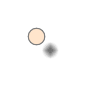
\begin{tikzpicture}
    \addtolength{\boxw}{\boxroundness * 2}
    \addtolength{\boxh}{\boxroundness * 2}

    \foreach \x in {0,.05,...,1}
    {
        \setlength{\tmpa}{\shadowsize * \real{\x}}
        \fill[xshift=\shadowsize - 1pt,yshift=-\shadowsize + 1pt,
                black,opacity=.04,rounded corners=\boxroundness]
            (\tmpa, \tmpa) rectangle +(\boxw - \tmpa - \tmpa,
                \boxh - \tmpa - \tmpa);
    }

    \filldraw[fill=lightorange, draw=black!50, rounded corners=\boxroundness]
        (0, 0) rectangle (\boxw, \boxh);
    \draw node[xshift=\boxroundness,yshift=\boxroundness,
        inner sep=1pt,outer sep=1pt,anchor=south west]
             (0,0) {\usebox{\shadowblockbox}};
\end{tikzpicture}}


%%%%%%%%5

\newcommand{\ceil}[1]{\left\lceil{#1}\right\rceil}

\newcommand{\optimize}[4]{%
  \begin{align}
    \min_{\substack{#2}}\quad & \label{opt:#1} #3 \\
    \text{subj. to}\quad & \nonumber #4
  \end{align}}

\newcommand{\optimizeoneline}[4]{%
  \begin{align}
    \min_{\substack{#2}}\quad & \label{opt:#1} #3 \quad
    \text{subj. to}\quad #4
  \end{align}}

\newcommand{\optimizemax}[4]{%
  \begin{align}
    \max_{\substack{#2}}\quad & \label{opt:#1} #3 \\
    \text{subj. to}\quad & \nonumber #4
  \end{align}}

\newcommand{\optimizemaxoneline}[4]{%
  \begin{align}
    \max_{\substack{#2}}\quad & \label{opt:#1} #3 \quad
    \text{subj. to}\quad #4
  \end{align}}

\newcommand{\optimizeuc}[3]{%
  \begin{align}
    \min_{\substack{#2}}\quad & \label{opt:#1} #3
  \end{align}}

\newcommand{\optimizeLagrange}[4]{%
  \begin{align}
    \max_{\substack{#2}} \min_{\substack{#3}}\quad & \label{opt:#1} #4
  \end{align}}

\newcommand{\optimizemaxuc}[3]{%
  \begin{align}
    \max_{\substack{#2}}\quad & \label{opt:#1} #3
  \end{align}}

\newcommand{\optimizemaxLagrange}[4]{%
  \begin{align}
    \min_{\substack{#2}} \max_{\substack{#3}}\quad & \label{opt:#1} #4
  \end{align}}

%\newtheorem{theorem}{Theorem}
%\newtheorem{definition}{Definitions}

%%% Local Variables: 
%%% mode: latex
%%% TeX-master: "courseml"
%%% End: 


\usepackage{times}
\usepackage[T1]{fontenc}
% Or whatever. Note that the encoding and the font should match. If T1
% does not look nice, try deleting the line with the fontenc.
\newcommand{\myalert}[1]{{%\color{red}
 #1}}
\iffalse
\begin{learningobjectives}
\item Explain the biological inspiration for multi-layer neural
  networks.
\item Construct a two-layer network that can solve the XOR problem.
\item Implement the back-propogation algorithm for training
  multi-layer networks.
\item Explain the trade-off between depth and breadth in network
  structure.
\item Contrast neural networks with radial basis functions with
  $k$-nearest neighbor learning.
\end{learningobjectives}

\dependencies{}

\newthought{The first learning models} you learned about (decision
trees and nearest neighbor models) created complex,
\concept{non-linear} decision boundaries.  We moved from there to the
perceptron, perhaps the most classic linear model.  At this point, we
will move \emph{back} to non-linear learning models, but using all
that we have learned about linear learning thus far.

This chapter presents an extension of perceptron learning to
non-linear decision boundaries, taking the biological inspiration of
neurons even further.  In the perceptron, we thought of the input data
point (e.g., an image) as being directly connected to an output (e.g.,
label).  This is often called a \concept{single-layer network} because
there is one layer of weights.  Now, instead of directly connecting
the inputs to the outputs, we will insert a layer of ``hidden'' nodes,
moving from a single-layer network to a \concept{multi-layer network}.
But introducing a non-linearity at inner layers, this will give us
non-linear decision boundaires.  In fact, such networks are able to
express almost any function we want, not just linear functions.  The
trade-off for this flexibility is increased complexity in parameter
tuning and model design.
\fi

\title[Neural Networks]
{Neural Networks}

\institute[] % (optional, but mostly needed)
{
%ENDIF -- University of Ferrara,  Italy\\
% fabrizio.riguzzi@unife.it
}
% - Use the \inst command only if there are several affiliations.
% - Keep it simple, no one is interested in your street address.
\date{}

\begin{document}
\begin{frame}
\titlepage 
\vspace{-2cm}
\begin{center}
Chapter 8 of ``A Course in  Machine Learning'' by Hal Daum\'e III

\url{http://ciml.info}

Conversion to beamer by Fabrizio Riguzzi
\end{center}


\end{frame}
  \renewcommand{\concept}[1]{\myalert{#1}}
  \renewcommand{\koncept}[2]{\myalert{#1}}

\renewcommand{\Figure}[3]{%
    \begin{center}
    \includegraphics[width=#3\textwidth]{../book/figs/#1}
    \end{center}
  }
  
\begin{frame}
  \frametitle{Bio-inspired Multi-Layer Network}
\begin{itemize}
\item 
One of the major weaknesses of linear models, like perceptron and the
regularized linear models from the previous chapter, is that they are unable to learn arbitrary decision
boundaries.
\item  In contrast, decision trees and $K$NN \emph{could} learn
arbitrarily complicated decision boundaries.
\end{itemize}
\end{frame}

\begin{frame}
  \frametitle{Bio-inspired Multi-Layer Network}
\begin{itemize}
\item 
One approach to doing this is to chain together a collection of
perceptrons to build more complex \concept{neural networks}. 
\item \concept{Two-layer network} 
\Figure{nnet:twolayer}{picture of a two-layer network with 5
  inputs and two hidden units}{0.4}
\end{itemize}
\end{frame}

\begin{frame}
  \frametitle{Bio-inspired Multi-Layer Network}
\begin{itemize}
\item Five inputs
(features) that are fed into two \concept{hidden units}.
\item  These hidden
units are then fed in to a single \concept{output unit}. 
\item
 Each edge in
this figure corresponds to a different weight.  
\item This is called a two-layer network
because we don't count the inputs as a real layer.  That is, it's two
layers of \emph{trained} weights.
\end{itemize}
\end{frame}

\begin{frame}
  \frametitle{Bio-inspired Multi-Layer Network}
\begin{itemize}
\item 
Prediction with a neural network is a straightforward generalization
of prediction with a perceptron. 
\item  First you compute activations of the
nodes in the hidden unit based on the inputs and the input weights.
\item Then you compute activations of the output unit given the hidden unit
activations and the second layer of weights.
\end{itemize}
\end{frame}

\begin{frame}
  \frametitle{Bio-inspired Multi-Layer Network}
\begin{itemize}
\item 
The only major difference  is that the hidden units compute a \emph{non-linear}
function of their inputs.  
\item 
This is usually called the
\concept{activation function} or \concept{link function}. 
\item If $w_{i,d}$ is the weights on the edge connecting input $d$
to hidden unit $i$, then the activation of hidden unit $i$ is computed
as:
%
\begin{equation}
  h_i = f\left( \dotp{\vw_i}{\vx} \right)
\end{equation}
%
Where $f$ is the link function and $\vw_i$ refers to the
vector of weights feeding in to node $i$.
\end{itemize}
\end{frame}

\begin{frame}
  \frametitle{Bio-inspired Multi-Layer Network}
\begin{itemize}
\item 
One example link function is the \concept{sign} function. 
\item If
the incoming signal is negative, the activation is $-1$.  Otherwise
the activation is $+1$.  
\item Problem: it
is non-differentiable.
\end{itemize}
\end{frame}

\begin{frame}
  \frametitle{Bio-inspired Multi-Layer Network}
\begin{itemize}
\item
A more popular link function is the \concept{hyperbolic tangent}
function, $\tanh$. 
\item Comparison between the sign function and the
$\tanh$ function 
\Figure{nnet:tanh}{picture of sign versus tanh}{0.3}
\item It
is a reasonable approximation to the sign function, but 
is differentiable.%\sidenote{It's derivative is just
  %$1-\tanh^2(x)$.}  
\item  Because it looks like an ``S'' and because the
Greek character for ``S'' is ``Sigma,'' such functions are usually
called \concept{sigmoid} functions.
\end{itemize}
\end{frame}

\begin{frame}
  \frametitle{Bio-inspired Multi-Layer Network}
\begin{itemize}
\item
Assuming for now that we are using $\tanh$ as the link function, the
overall prediction made by a two-layer network can be computed using
\end{itemize}
\newalgorithm%
  {nnet:twolayerpredict}%
  {\FUN{TwoLayerNetworkPredict}(\VAR{$\mat W$}, \VAR{$\vec v$}, \VAR{$\hat\vx$})}
  {
\FOR{\VAR{i} = \CON{1} \TO \VAR{number of hidden units}}
\SETST{$h_i$}{$\tanh(\dotp{\VARm{\vec w_i}}{\VARm{\hat\vx}})$}
\COMMENT{compute activation of hidden unit $i$}
\ENDFOR
\RETURN $\dotp{\VARm{\vec v}}{\VARm{\vec h}}$
\COMMENT{compute output unit}
}
\end{frame}

\begin{frame}
  \frametitle{Bio-inspired Multi-Layer Network}
\begin{itemize}
\item The function takes a
matrix of weights $\mat W$ corresponding to the first layer weights
and a vector of weights $\vec v$ corresponding to the second layer.
\item
You can write this entire computation out in one line as:
%
\begin{align}
\hat y
&= \sum_i v_i \tanh( \dotp{\vec w_i}{\hat\vx} ) \\
&= \dotp{\vec v}{\tanh( \mat W \hat\vx )} \label{eq:nnet:matrixeq}
\end{align}
%
where we assume that $\tanh$ takes a
vector as input and produces a vector as output.
\end{itemize}
\end{frame}

\begin{frame}
  \frametitle{Bio-inspired Multi-Layer Network}
\begin{itemize}
%\thinkaboutit{Is it necessary to use a link function at all?  What
%  would happen if you just used the identify function as a link?}
\item
The claim is that two-layer neural networks are more expressive than
single layer networks (i.e., perceptrons).
\item We construct a very small two-layer network for solving the XOR problem.
\item
Small XOR data set:
\begin{tabular}{r|rrr}
  $y$ & $x_0$ & $x_1$ & $x_2$ \\
  \hline
  -1 & +1 & +1 & +1 \\
  -1 & +1 & -1 & -1 \\
  +1 & +1 & +1 & -1 \\
  +1 & +1 & -1 & +1
\end{tabular}
\item $x_0$ is a dummy feature used to take into account the bias.
\item The classification rule is
that $y=+1$ if an only if $x_1=\neg x_2$, where the features are just $\pm
1$.
\end{itemize}
\end{frame}

\begin{frame}
  \frametitle{Bio-inspired Multi-Layer Network}
\begin{itemize}
\item
You can solve this problem using a two layer network with two hidden
units.
\item  The key idea is to make the first hidden unit compute an
``or'' function: $x_1 \lor x_2$. 
\item The second hidden unit can compute
an ``and'' function: $x_1 \land x_2$. 
\item The the output can combine
these into a single prediction that mimics XOR. 
\item  Once you have the
first hidden unit activate for ``or'' and the second for ``and,'' you
need only set the output weights as $+1$ and $-2$, respectively.
\end{itemize}
\end{frame}

\begin{frame}
  \frametitle{Bio-inspired Multi-Layer Network}
\begin{itemize}
\item
%\thinkaboutit{Verify that these output weights will actually give you XOR.}
To achieve the ``or'' behavior, you can start by setting the bias to
$-0.5$ and the weights for the two ``real'' features as both being
$1$.
\item This will do the ``right thing''
if the link function were the sign function.
\item  To get $\tanh$ to mimic $\sign$, you need to make the dot
product either really really large or really really small.  
\item You can
accomplish this by setting the bias to $-500,000$ and both of the two
weights to $1,000,000$.
\item  Now, the activation of this unit will be just
slightly above $-1$ for $\vx = \langle -1,-1 \rangle$ and just
slightly below $+1$ for the other three examples.
\end{itemize}
\end{frame}

\begin{frame}
  \frametitle{Bio-inspired Multi-Layer Network}
\begin{itemize}
%\thinkaboutit{This shows how to create an ``or'' function.  How can
%  you create an ``and'' function?}
\item
Do you get additional
representational power by moving beyond two layers?  
\item The answer is
partially provided in the following Theorem, due originally to George
Cybenko for one particular type of link function, and extended later
by Kurt Hornik to arbitrary link functions.
\begin{theorem}[Two-Layer Networks are Universal Function Approximators] \label{thm:nnet:twolayer}
%
  Let $F$ be a continuous function on a bounded subset of
  $D$-dimensional space.  Then there exists a two-layer neural network
  $\hat F$ with a finite number of hidden units that approximate $F$
  arbitrarily well.  Namely, for all $\vx$ in the domain of $F$,
  $\ab{F(\vx) - \hat F(\vx)} < \ep$.
\end{theorem}
\item
Or, in colloquial terms ``two-layer networks can approximate any
function.''
\end{itemize}
\end{frame}

\begin{frame}
  \frametitle{Bio-inspired Multi-Layer Network}
\begin{itemize}
\item
This theorem  says that if you give
me a function $F$ and some error tolerance parameter $\ep$, I can
construct a two layer network that computes $F$. 
\item Going from one layer to two layers completely changes the
representational capacity of your model.
\end{itemize}
\end{frame}

\begin{frame}
  \frametitle{Bio-inspired Multi-Layer Network}
\begin{itemize}
\item
How many
hidden units should I have?  
\item If your data is $D$ dimensional and you
have $K$ hidden units, then the total number of parameters is
$(D+2)K$.
\item   The first $+1$ is from the bias, the second is from the
second layer of weights.
\item   Heuristic: you
should have one to two examples for each parameter you are trying to
estimate.
\item Choose the number of hidden
units as roughly $\lfloor \frac N D \rfloor$.  
\end{itemize}
\end{frame}

\begin{frame}
  \frametitle{Bio-inspired Multi-Layer Network}
\begin{itemize}
\item
If you
have tons and tons of examples, you can safely have lots of hidden
units.  If you only have a few examples, you should probably restrict
the number of hidden units in your network.
\item 
The number of units is both a form of inductive bias and a form of
regularization. 
\item The number of hidden units controls how
complex your function will be.
\item  Lots of hidden units $\Rightarrow$
very complicated function. 
\item  As the number of hidden units increases, training performance continues
to get better.  But at some point, test performance gets worse because
the network has overfit the data.
\end{itemize}
\end{frame}
%\section{The Back-propagation Algorithm}

\begin{frame}
  \frametitle{The Back-propagation Algorithm}
\begin{itemize}
\item
The back-propagation algorithm is a classic approach to training
neural networks. 
\item You can summarize
back-propagation as:
%
\begin{equation}
\text{back-propagation} = \text{gradient descent} + \text{chain rule}
\end{equation}
%
\item You are going to optimize the weights in the network to minimize some
objective function.
\item  The only difference is that the predictor is no
longer linear (i.e., $\hat y = \dotp{\vw}{\vx}+b$) but now non-linear
(i.e., $\dotp{\vec v}{\tanh( \mat W \hat\vx )}$).
\item  The only question
is how to do gradient descent on this more complicated objective.
\end{itemize}
\end{frame}

\begin{frame}
  \frametitle{The Back-propagation Algorithm}
\begin{itemize}
\item
For now, we will ignore the idea of regularization.  
\item \emph{Historically}, neural networks have not been
regularized.  
\item Instead, people have used \concept{early stopping} as a
method for controlling overfitting.  
\item Presently, it's not obvious which
is a better solution: both are valid options.
\item We focus on optimizing squared error, mostly for historic reasons.
\item   You could easily replace
squared error with your loss function of choice.  
\end{itemize}
\end{frame}

\begin{frame}
  \frametitle{The Back-propagation Algorithm}
\begin{itemize}
\item
Our overall
objective is:
%
\optimizeuc{nnet:twolayer}{\mat W,\vec v}{%
  \sum_n \frac 1 2 \left( \textcolor{darkblue}{y_n - 
     \sum_i v_i f(\dotp{\vec w_i}{\vx_n})}
     \right)^2}
%
Here, $f$ is some link function like $\tanh$.
\end{itemize}
\end{frame}

\begin{frame}
  \frametitle{The Back-propagation Algorithm}
\begin{itemize}
\item
The easy case is to differentiate this with respect to $\vec v$: the
weights for the output unit.
\item  Without even doing any math, you should
be able to guess what this looks like.  
\item From $\vec v$s perspective, it is just a linear model, attempting
to minimize squared error. 
\item The only ``funny'' thing is that its
inputs are the activations $\vec h$ rather than the examples $\vx$.
\item So the gradient with respect to $\vec v$ is just as for the linear
case.
\end{itemize}
\end{frame}

\begin{frame}
  \frametitle{The Back-propagation Algorithm}
\begin{itemize}
\item
Let $e_n$ denote the
\emph{error} on the $n$th example (i.e., the blue term above), and let
$\vec h_n$ denote the vector of hidden unit activations on that
example.  Then:
%
\begin{equation}
\grad_{\vec v} = -\sum_n e_n \vec h_n 
\end{equation}
%
\item This is exactly like the linear case. 
\item  One way of interpreting this
is: how would the output weights have to change to make the prediction
better?  This is an easy question to answer because they can easily
measure how their changes affect the output.
\end{itemize}
\end{frame}

\begin{frame}
  \frametitle{The Back-propagation Algorithm}
\begin{itemize}
\item
The more complicated aspect to deal with is the weights corresponding
to the \emph{first} layer.
\item   The reason this is difficult is because
the weights in the first layer aren't necessarily trying to produce
specific values, say $0$ or $5$ or $-2.1$. 
\item They are simply trying to
produce activations that get fed to the output layer.  So the change
they want to make depends crucially on how the output layer interprets
them.
\end{itemize}
\end{frame}

\begin{frame}
  \frametitle{The Back-propagation Algorithm}
\begin{itemize}
\item
Thankfully, the chain rule of calculus saves us.  Ignoring the sum
over data points, we can compute:
%
\begin{align}
\cL(\mat W) &= 
\frac 1 2 \left( \textcolor{darkblue}{y - 
     \sum_i v_i f(\dotp{\vec w_i}{\vx})}
     \right)^2
\\
\frac {\partial \cL} {\partial \vec w_i}
&= \frac {\partial \cL} {\partial f_i}
   \frac {\partial f_i}   {\partial \vec w_i}
\\
\frac {\partial \cL} {\partial f_i}
&= -\left(y - \sum_i v_i f(\dotp{\vec w_i}{\vx})\right) v_i
= -e v_i
\\
\frac {\partial f_i} {\partial \vec w_i}
&= f'(\dotp{\vec w_i}{\vx}) \vx
\end{align}
%
\end{itemize}
\end{frame}

\begin{frame}
  \frametitle{The Back-propagation Algorithm}
\begin{itemize}
\item
Putting this together, we get that the gradient with respect to
$\vw_i$ is:
%
\begin{equation}
\grad_{\vw_i}
= -e v_i f'(\dotp{\vw_i}{\vx}) \vec x
\end{equation}
%
\item  If the overall error of the
predictor ($e$) is small, you want to make small steps.  
\item If $v_i$ is
small for hidden unit $i$, then this means that the output is not
particularly sensitive to the activation of the $i$th hidden unit.
\item 
Thus, its gradient should be small.  If $v_i$ flips sign, the gradient
at $\vw_i$ should also flip sign.
\item  The name
\concept{back-propagation} comes from the fact that you propagate
gradients backward through the network, starting at the end.
\end{itemize}
\end{frame}

\begin{frame}
  \frametitle{The Back-propagation Algorithm}
  \begin{scriptsize}
\FUN{TwoLayerNetworkTrain}(\VAR{$\mat D$}, \VAR{$\eta$}, \VAR{K}, \VAR{MaxIter})
 \begin{algorithmic}[1]
\SETST{$\mat W$}{$D \times K$ matrix of small random values}
\COMMENT{initialize input layer weights}
\SETST{$\vec v$}{$K$-vector of small random values}
\COMMENT{initialize output layer weights}
\FOR{\VAR{iter} = \CON{1} \dots \VAR{MaxIter}}
\SETST{$\mat G$}{$D \times K$ matrix of zeros}
\COMMENT{initialize input layer gradient}
\SETST{$\vec g$}{$K$-vector of zeros}
\COMMENT{initialize output layer gradient}
\FORALL{(\VAR{$\vx$},\VAR{$y$}) $\in$ \VAR{$\mat D$}}
\FOR{\VAR{i} = \CON{1} \TO \VAR{K}}
\SETST{$a_i$}{$\dotp{\VARm{\vec w_i}}{\VARm{\hat\vx}}$}
\SETST{$h_i$}{$\tanh(\VARm{a_i})$}
\COMMENT{compute activation of hidden unit $i$}
\ENDFOR
\SETST{$\hat y$}{$\dotp{\VARm{\vec v}}{\VARm{\vec h}}$}
\COMMENT{compute output unit}
\SETST{$e$}{$\VARm{y} - \VARm{\hat y}$}
\COMMENT{compute error}
\SETST{$\vec g$}{$\VARm{\vec g} - \VARm{e} \VARm{\vec h}$}
\COMMENT{update gradient for output layer}
\FOR{\VAR{i} = \CON{1} \TO \VAR{K}}
\SETST{$\mat G_i$}{$\VARm{\mat G_i} - \VARm{e} \VARm{v_i} (\CON{1} - \tanh^2(\VARm{a_i})) \VARm{\vx}$}
\COMMENT{update gradient for input layer}
\ENDFOR
\ENDFOR
\SETST{$\mat W$}{$\VARm{\mat W} - \VARm{\eta} \VARm{\mat G}$}
  \COMMENT{update input layer weights}
\SETST{$\vec v$}{$\VARm{\vec v} - \VARm{\eta} \VARm{\vec g}$}
  \COMMENT{update output layer weights}
\ENDFOR
\RETURN \VAR{$\mat W$}, \VAR{$\vec v$}
      \end{algorithmic}  
\end{scriptsize}
\end{frame}

\begin{frame}
  \frametitle{The Back-propagation Algorithm}
\begin{itemize}
\item 
%\thinkaboutit{What would happen to this algorithm if you wanted to
%  optimize exponential loss instead of squared error?  What if you
%  wanted to add in weight regularization?}
Implementing the back-propagation
algorithm can be a bit tricky. 
\item Sign errors often abound.  
\item A useful
trick is first to keep $\mat W$ fixed and work on just training $\vec
v$.  
\item Then keep $\vec v$ fixed and work on training $\mat W$.  Then put
them together.
\end{itemize}
\end{frame}
%\thinkaboutit{If you like matrix calculus, derive the same algorithm
%  starting from Eq~\eqref{eq:nnet:matrixeq}.}

%\section{Initialization and Convergence of Neural Networks}

\begin{frame}
  \frametitle{Initialization and Convergence of Neural Networks}
\begin{itemize}
\item
You might be tempted to
initialize all the weights in a neural network to zero. 
\item  In the algorithm they're initialized to small random values 
because an initialization of $\mat W = \mat 0$ and $\vec
v = \vec 0$ will lead to ``uninteresting'' solutions.  
\item If you initialize the model in this way, it remains stuck
in that situation, which is a bad local optimum.  
\item On any
example $\vx$, the activation $h_i$ of the hidden units will all be
zero since $\mat W = \mat 0$. 
\item This means that on the first iteration,
the gradient on the output weights ($\vec v$) will be zero, so they
will stay put. 
\end{itemize}
\end{frame}

\begin{frame}
  \frametitle{Initialization and Convergence of Neural Networks}
\begin{itemize}
\item The gradient of the weights of the hidden units will also be zero
\item So 
all the weights will remain  zero through the whole algorithm, leading to 
an uninteresting solution
\end{itemize}
\end{frame}

\begin{frame}
  \frametitle{Initialization and Convergence of Neural Networks}
\begin{itemize}
\item Now suppose the weights $\vec v$ are initialized to the same nonzero value and the weights 
vectors $\vec w_i$ are initialized
so that $\vec w_i=\vec w_j$ for $i,j$ hidden units
\item In this case the components of the gradient for $\vec v$ will all be the same 
\item Similarly, the gradient for the $d$th
feature on the first unit $w_{1,d}$ will be \emph{exactly} the same as the
gradient $w_{2,d}$ for the same feature on the second unit.  
\item This
means that the weight matrix, after a gradient step, will change in
\emph{exactly the same way} for every hidden unit. 
\end{itemize}
\end{frame}

\begin{frame}
  \frametitle{Initialization and Convergence of Neural Networks}
\begin{itemize} 
\item Thinking through
this example for iterations $2\dots$, the values of the hidden units
will \emph{always} be exactly the same, which means that the weights
feeding in to any of the hidden units will be exactly the same.
\item
Eventually the model will converge, but it will converge to a solution
that does not take advantage of having access to the hidden units.
\end{itemize}
\end{frame}

\begin{frame}
  \frametitle{Initialization and Convergence of Neural Networks}
\begin{itemize}
\item
Neural networks are \emph{sensitive} to their
initialization.
\item The function that they optimize is
\concept{non-convex}, meaning that it might have plentiful local
optima.  (One of which is the trivial local optimum described in the
preceding slide.)  
\end{itemize}
\end{frame}

\begin{frame}
  \frametitle{Initialization and Convergence of Neural Networks}
\begin{itemize}
\item Neural networks \emph{must} have
local optima.  
\item Suppose you have a two layer network with two hidden
units that's been optimized. 
\item You have weights $\vw_1$ from inputs to
the first hidden unit, weights $\vw_2$ from inputs to the second
hidden unit and weights $(v_1,v_2)$ from the hidden units to the
output.
\item  If I give you back another network with $\vw_1$ and $\vw_2$
swapped, and $v_1$ and $v_2$ swapped, the network computes
\emph{exactly} the same thing, but with a markedly different weight
structure. 
\item This phenomena is known as \concept{symmetric modes}
(``mode'' referring to an optima) meaning that there are symmetries in
the weight space. 
\end{itemize}
\end{frame}

\begin{frame}
  \frametitle{Initialization and Convergence of Neural Networks}
\begin{itemize}
\item  It would be one thing if there were lots of modes
and they were all symmetric: then finding one of them would be as good
as finding any other.
\item  Unfortunately there are additional local
optima that are \emph{not} global optima.
\end{itemize}
\end{frame}

\begin{frame}
  \frametitle{Initialization and Convergence of Neural Networks}
\begin{itemize}
\item
Random initialization of the weights of a network is a way to address
\emph{both} of these problems.  
\item By initializing a network with small
random weights (say, uniform between $-0.1$ and $0.1$), the network is
unlikely to fall into the trivial, symmetric local optimum.  
\item Moreover,
by training a collection of networks, each with a different random
initialization, you can often obtain better solutions that with just
one initialization. 
\item In other words, you can train ten networks with
different random seeds, and then pick the one that does best on
held-out data. 
\end{itemize}
\end{frame}

\begin{frame}
  \frametitle{Initialization and Convergence of Neural Networks}
\Figure{nnet:converge}{convergence of randomly initialized networks}{0.4}
\begin{itemize}
\item
Prototypical
\emph{test-set} performance for ten networks with different random
initialization, plus an eleventh plot for the trivial symmetric
network initialized with zeros.
\end{itemize}
\end{frame}

\begin{frame}
  \frametitle{Initialization and Convergence of Neural Networks}
\begin{itemize}
\item
One of the typical complaints about neural networks is that they are
finicky.  In particular, they have a rather large number of knobs to
tune:
%
\begin{enumerate}
\item The number of layers
\item The number of hidden units per layer
\item The gradient descent learning rate $\eta$
\item The initialization
\item The stopping iteration or weight regularization
\end{enumerate}
%
\item The last of these is minor (early stopping is an easy regularization
method that does not require much effort to tune).
\item  Even for two layer networks, having to choose
the number of hidden units, and then get the learning rate and
initialization ``right'' can take a bit of work.  Clearly it can be
automated, but nonetheless it takes time.
\end{itemize}
\end{frame}

\begin{frame}
  \frametitle{Initialization and Convergence of Neural Networks}
\begin{itemize}
\item
Another difficulty of neural networks is that their weights can be
difficult to interpret. 
\item  For linear networks, you
can often interpret high weights as indicative of positive examples
and low weights as indicative of negative examples.  
\item In multilayer
networks, it becomes very difficult to try to understand what the
different hidden units are doing.  
\end{itemize}
\end{frame}

%TODO: maybe have something about doing images?


%\section{Beyond Two Layers}
\begin{frame}
  \frametitle{Beyond Two Layers}
\begin{itemize}
\item
The definition of neural networks and the back-propagation algorithm
can be generalized beyond two layers to any arbitrary directed acyclic
graph. 
\item In practice, it is most common to use a layered network unless one has a very
strong reason (aka inductive bias) to do something different.
\Figure{nnet:layered}{multi-layer network}{0.35}
\end{itemize}
\end{frame}

\begin{frame}
  \frametitle{Beyond Two Layers}
\begin{itemize}
\item
The view as a directed graph sheds a different sort of
insight on the back-propagation algorithm.
\item Suppose that your network structure is stored in some directed acyclic
graph
\Figure{nnet:dag}{DAG network}{0.35}
\end{itemize}
\end{frame}

\begin{frame}
  \frametitle{Beyond Two Layers}
\begin{itemize}
\item
 We index nodes in this
graph as $u,v$.  
\item The activation \emph{before} applying non-linearity
at a node is $a_u$ and after non-linearity is $h_u$.  
\item The graph has a
single sink, which is the output node $y$ with activation $a_y$ (no
non-linearity is performed on the output unit). 
\item  The graph has
$D$-many inputs (i.e., nodes with no parent), whose activations $h_u$
are given by an input example.  
\item An edge $(u,v)$ is from a parent to a
child (i.e., from an input to a hidden unit, or from a hidden unit to
the sink). 
\item Each edge has a weight $w_{u,v}$.  We say that
$\textit{par}(u)$ is the set of parents of $u$.
\end{itemize}
\end{frame}

\begin{frame}
  \frametitle{Beyond Two Layers}
\begin{itemize}
\item
There are two relevant algorithms: forward-propagation and
back-propagation.
\item  Forward-propagation tells you how to compute the
activation of the sink $y$ given the inputs.  
\item Back-propagation
computes derivatives of the edge weights for a given input.
\end{itemize}
\end{frame}

\begin{frame}
  \frametitle{Beyond Two Layers}
\newalgorithm%
  {nnet:forwardprop}%
  {\FUN{ForwardPropagation}{($\vx$)}}
  {
\FORALL{input nodes $u$}
\SETST{$h_u$}{corresponding feature of $\vx$}
\ENDFOR
\FORALL{nodes $v$ in the network whose parent's are computed}
\SETST{$a_v$}{$\sum_{u \in \textit{par}(v)} w_{(u,v)} h_u$}
\SETST{$h_v$}{$\tanh(a_v)$}
\ENDFOR
\RETURN $a_y$
}
\end{frame}

\begin{frame}
  \frametitle{Beyond Two Layers}
\newalgorithm%
  {nnet:backprop}%
  {\FUN{BackPropagation}{($\vx$, $y$)}}
  {
\STATE{run \FUN{ForwardPropagation}(\VAR{$\vx$}) to compute activations}
\SETST{$e_y$}{$y - a_y$}
  \COMMENT{compute overall network error}
\FORALL{nodes $v$ in the network whose error $e_v$ is computed}
\FORALL{$u \in \textit{par}(v)$}
\SETST{$g_{u,v}$}{$- e_v h_u$}
  \COMMENT{compute gradient of this edge}
\SETST{$e_u$}{$e_u + e_v w_{u,v} (1 - \tanh^2(a_u))$}
  \COMMENT{compute the ``error'' of the parent node}
\ENDFOR
\ENDFOR
\RETURN all gradients $g_e$
}
\end{frame}

\begin{frame}
  \frametitle{Beyond Two Layers}
\begin{itemize}
\item
The key aspect of the \concept{forward-propagation} algorithm is to
iteratively compute activations, going deeper and deeper in the DAG.
\item Once the activations of all the parents of a node $u$ have been
computed, you can compute the activation of node $u$.  
\Figure{nnet:forwardprop}{picture of forward prop}{0.4}
\end{itemize}
\end{frame}

\begin{frame}
  \frametitle{Beyond Two Layers}
\begin{itemize}
\item
Back-propagation does the
opposite: it computes gradients top-down in the network.
\item  The key idea
is to compute an \emph{error} for each node in the network.  
\item The error
at the output unit is the ``true error.''
\item   For any hidden unit, the
error is the amount of gradient that we see coming from our children
(i.e., higher in the network).
\item  These errors are computed backwards in
the network (hence the name \concept{back-propagation}) along with the
gradients themselves.
\end{itemize}
\end{frame}

\begin{frame}
  \frametitle{Beyond Two Layers}
\Figure{nnet:backprop}{picture of back prop}{0.4}
\begin{itemize}
\item
Given the back-propagation algorithm, you can directly run gradient
descent, using it as a subroutine for computing the gradients.
\end{itemize}
\end{frame}

%\section{Breadth versus Depth}

\begin{frame}
  \frametitle{Breadth versus Depth}
\begin{itemize}
\item
If two-layer networks are so great, why do we care about
deeper networks?
\item
We can borrow some ideas from CS theory,
namely the idea of \concept{circuit complexity}.  
\item There are functions for which it might be a ``good idea'' to use
a deep network. 
\item  There are functions that will require
a huge number of hidden units if you force the network to be shallow,
but can be done in a small number of units if you allow it to be
deep. 
\item  The example that we'll use is the \concept{parity function}
which, ironically enough, is just a generalization of the XOR
problem.
\end{itemize}
\end{frame}

\begin{frame}
  \frametitle{Breadth versus Depth}
\begin{itemize}
\item
  The function is defined over binary inputs as:
%
\begin{align}
\textit{parity}(\vx)
&= \sum_d x_d \mod 2 \\
&= \brack{ 1 & \text{if the number of $1$s in $\vx$ is odd} \\
           0 & \text{if the number of $1$s in $\vx$ is even} }
\end{align}
%
%\TODOFigure{nnet:paritydeep}{deep function for computing parity}
%
\item It is easy to define a circuit of depth $\cO(\log_2 D)$ with
$\cO(D)$-many gates for computing the parity function.
\item  Each gate is
an XOR, arranged in a complete binary tree
\item If you want to disallow XOR as a
gate, you can fix this by allowing the depth to be doubled and
replacing each XOR with an AND, OR and NOT combination
\end{itemize}
\end{frame}

\begin{frame}
  \frametitle{Breadth versus Depth}
\begin{itemize}
\item
This shows that if you are allowed to be deep, you can construct a
circuit  that computes parity using a number of hidden units that
is linear in the dimensionality.
\item   Can you do the same with shallow
circuits?  The answer is no. 
\item  It's a famous result of circuit
complexity that parity requires exponentially many gates to compute in
constant depth.  The formal theorem is below:
\begin{theorem}[Parity Function Complexity] \label{thm:nnet:parity}
  Any circuit of depth $K < \log_2 D$ that computes the parity
  function of $D$ input bits must contain $\cO(e^D)$ gates.
\end{theorem}
\end{itemize}
\end{frame}

\begin{frame}
  \frametitle{Breadth versus Depth}
\begin{itemize}
\item
This is a very famous result because it shows that constant-depth
circuits are less powerful that deep circuits.  
\item Although a neural
network isn't exactly the same as a circuit, it is generally believed
that the same result holds for neural networks.
\item  At the very least,
this gives a strong indication that depth might be an important
consideration in neural networks.
\end{itemize}
\end{frame}

%\thinkaboutit{What is it about neural networks that makes it so that
%  the theorem about circuits does not apply directly?}

\begin{frame}
  \frametitle{Breadth versus Depth}
\begin{itemize}
\item
One way of thinking about the issue of breadth versus depth has to do
with the number of \emph{parameters} that need to be estimated.  
\item By
the heuristic that you need roughly one or two examples for every
parameter, a deep model could potentially require exponentially fewer
examples to train than a shallow model!
\end{itemize}
\end{frame}

\begin{frame}
  \frametitle{Breadth versus Depth}
\begin{itemize}
\item
This now flips the question: if deep is potentially so much better,
why doesn't everyone use deep networks? 
\item   First, it makes the \concept{architecture selection} problem
more significant.
\item When you use a two-layer network, the only
hyperparameter to choose is how many hidden units should go in the
middle layer.
\item  When you choose a deep network, you need to choose how
many layers, and what is the width of all those layers.  This can be
somewhat daunting.
\end{itemize}
\end{frame}

\begin{frame}
  \frametitle{Breadth versus Depth}
\begin{itemize}
\item
A second issue has to do with training deep models with
back-propagation. 
\item  As back-propagation works its way down
through the model, the sizes of the gradients shrink.
\item   If you are at the
beginning of a very deep network, changing one single weight is
unlikely to have a significant effect on the output, since it has to
go through so many other units before getting there. 
\item  This directly
implies that the derivatives are small.  
\item This, in turn, means that
back-propagation essentially never moves far from its initialization
when run on very deep networks.
\end{itemize}
\end{frame}

\begin{frame}
  \frametitle{Breadth versus Depth}
\begin{itemize}
\item
%\thinkaboutit{While these small derivatives might make training
%  difficult, they might be \emph{good} for other reasons: what
%  reasons?}
Finding good ways to train deep networks is an active research area.
\item There are two general strategies. 
\item The first is to attempt to
initialize the weights better, often by a \concept{layer-wise}
initialization strategy. 
\item This can be often done using unlabeled data.
\item After this initialization, back-propagation can be run to tweak the
weights for whatever classification problem you care about.  
\end{itemize}
\end{frame}

\begin{frame}
  \frametitle{Breadth versus Depth}
\begin{itemize}
\item
A second
approach is to use a more complex optimization procedure, rather than
gradient descent.  
\end{itemize}
\end{frame}

%\section{Basis Functions}

\begin{frame}
  \frametitle{Basis Functions}
\begin{itemize}
\item
 (a) neural networks can mimic linear
functions and (b) they can learn more complex functions.  
\item A reasonable
question is whether they can mimic a $K$NN classifier, and whether
they can do it efficiently (i.e., with not-too-many hidden units).
\item 
A natural way to train a neural network to mimic a $K$NN classifier is
to replace the sigmoid link function with a \concept{radial basis
  function} (RBF).
\item  In a \concept{sigmoid network} (i.e., a network
with sigmoid links), the hidden units were computed as $h_i =
\tanh(\dotp{\vw_i,\vx})$.
\item  In an \concept{RBF network}, the hidden
units are computed as:
%
\begin{equation}
h_i = \exp\left[ - \ga_i \norm{\vw_i - \vx}^2 \right]
\end{equation}
%
%\TODOFigure{nnet:rbfpicture}{a one-D picture of RBF bumps}
%\TODOFigure{nnet:unitsymbols}{picture of nnet with sigmoid/rbf units}
%
\end{itemize}
\end{frame}

\begin{frame}
  \frametitle{Basis Functions}
\begin{itemize}
\item
The hidden units behave like little Gaussian ``bumps''
centered around locations specified by the vectors $\vw_i$.  
\item The parameter $\ga_i$ specifies the \emph{width} of the Gaussian bump.
\item If $\ga_i$ is large, then only data points that are really close to
$\vw_i$ have non-zero activations.  
\item To distinguish sigmoid networks
from RBF networks, the hidden units are typically drawn with sigmoids
or with Gaussian bumps.
\end{itemize}
\end{frame}

%\section{Basis Functions}

\begin{frame}
  \frametitle{Basis Functions}
\begin{itemize}
\item
Training RBF networks involves finding good values for the Gassian
widths, $\ga_i$, the centers of the Gaussian bumps, $\vw_i$ and the
connections between the Gaussian bumps and the output unit, $\vec v$.
\item This can all be done using back-propagation. 
\item The gradient terms for
$\vec v$ remain unchanged from before, the derivates for the other
variables differ 
\end{itemize}
\end{frame}

\begin{frame}
  \frametitle{Basis Functions}
\begin{itemize}
\item
One of the big questions with RBF networks is: where should the
Gaussian bumps be centered? 
\item  One can, of course, apply
back-propagation to attempt to find the centers. 
\item Another option is to
specify them ahead of time.
\end{itemize}
\end{frame}

\begin{frame}
  \frametitle{Basis Functions}
\begin{itemize}
\item One potential approach is
to have one RBF unit per data point, centered on that data point. 
\item If
you carefully choose the $\ga$s and $\vec v$s, you can obtain
something that looks nearly identical to distance-weighted $K$NN by
doing so. 
\item This has the added advantage that you can go futher, and
use back-propagation to \emph{learn} good Gaussian widths ($\ga$) and
``voting'' factors ($\vec v$) for the nearest neighbor algorithm.
%\thinkaboutit{Consider an RBF network with one hidden unit per
%  training point, centered at that point.  What bad thing might happen
%  if you use back-propagation to estimate the $\ga$s and $\vec v$ on
%  this data if you're not careful?  How could you be careful?}
%\item If you use \emph{fewer} hidden units than data points, you can think
% of this technique as a \concept{locally weighted linear model}.
%\item As with all neural networks,
% choosing the right number of hidden units (aka the
% \concept{architecture selection} problem) is one of the challenges
% in RBF network and locally weighted linear models.
\end{itemize}
\end{frame}


\end{document}
\begin{comment}
   - Multilayer perceptron
   - From linear to non-linear
   - Architecture choice
   - Basis functions
   - Each training point as a basic function
\end{comment}

\begin{exercises}
\begin{Ex}
\TODO

\begin{solution}
\TODO
\end{solution}
\end{Ex}

\end{exercises}

%%% Local Variables: 
%%% mode: latex
%%% TeX-master: "courseml"
%%% End: 
